\documentclass[12pt,letterpaper]{article}
\usepackage{graphicx,textcomp}
\usepackage{natbib}
\usepackage{setspace}
\usepackage{fullpage}
\usepackage{color}
\usepackage[reqno]{amsmath}
\usepackage{amsthm}
\usepackage{fancyvrb}
\usepackage{amssymb,enumerate}
\usepackage[all]{xy}
\usepackage{endnotes}
\usepackage{lscape}
\newtheorem{com}{Comment}
\usepackage{float}
\usepackage{hyperref}
\newtheorem{lem} {Lemma}
\newtheorem{prop}{Proposition}
\newtheorem{thm}{Theorem}
\newtheorem{defn}{Definition}
\newtheorem{cor}{Corollary}
\newtheorem{obs}{Observation}
\usepackage[compact]{titlesec}
\usepackage{dcolumn}
\usepackage{tikz}
\usetikzlibrary{arrows}
\usepackage{multirow}
\usepackage{xcolor}
\newcolumntype{.}{D{.}{.}{-1}}
\newcolumntype{d}[1]{D{.}{.}{#1}}
\definecolor{light-gray}{gray}{0.65}
\usepackage{url}
\usepackage{listings}
\usepackage{color}

\definecolor{codegreen}{rgb}{0,0.6,0}
\definecolor{codegray}{rgb}{0.5,0.5,0.5}
\definecolor{codepurple}{rgb}{0.58,0,0.82}
\definecolor{backcolour}{rgb}{0.95,0.95,0.92}

\lstdefinestyle{mystyle}{
	backgroundcolor=\color{backcolour},   
	commentstyle=\color{codegreen},
	keywordstyle=\color{magenta},
	numberstyle=\tiny\color{codegray},
	stringstyle=\color{codepurple},
	basicstyle=\footnotesize,
	breakatwhitespace=false,         
	breaklines=true,                 
	captionpos=b,                    
	keepspaces=true,                 
	numbers=left,                    
	numbersep=5pt,                  
	showspaces=false,                
	showstringspaces=false,
	showtabs=false,                  
	tabsize=2
}
\lstset{style=mystyle}
\newcommand{\Sref}[1]{Section~\ref{#1}}
\newtheorem{hyp}{Hypothesis}

\title{Problem Set 3}
\date{Due: March 26, 2023 - Marcus Ó Faoláin 16327268}
\author{Applied Stats II} 


\begin{document}
	\maketitle
	\section*{Instructions}
	\begin{itemize}
	\item Please show your work! You may lose points by simply writing in the answer. If the problem requires you to execute commands in \texttt{R}, please include the code you used to get your answers. Please also include the \texttt{.R} file that contains your code. If you are not sure if work needs to be shown for a particular problem, please ask.
\item Your homework should be submitted electronically on GitHub in \texttt{.pdf} form.
\item This problem set is due before 23:59 on Sunday March 26, 2023. No late assignments will be accepted.
	\end{itemize}

	\vspace{.25cm}
\section*{Question 1}
\vspace{.25cm}
\noindent We are interested in how governments' management of public resources impacts economic prosperity. Our data come from \href{https://www.researchgate.net/profile/Adam_Przeworski/publication/240357392_Classifying_Political_Regimes/links/0deec532194849aefa000000/Classifying-Political-Regimes.pdf}{Alvarez, Cheibub, Limongi, and Przeworski (1996)} and is labelled \texttt{gdpChange.csv} on GitHub. The dataset covers 135 countries observed between 1950 or the year of independence or the first year forwhich data on economic growth are available ("entry year"), and 1990 or the last year for which data on economic growth are available ("exit year"). The unit of analysis is a particular country during a particular year, for a total $>$ 3,500 observations. 

\begin{itemize}
	\item
	Response variable: 
	\begin{itemize}
		\item \texttt{GDPWdiff}: Difference in GDP between year $t$ and $t-1$. Possible categories include: "positive", "negative", or "no change"
	\end{itemize}
	\item
	Explanatory variables: 
	\begin{itemize}
		\item
		\texttt{REG}: 1=Democracy; 0=Non-Democracy
		\item
		\texttt{OIL}: 1=if the average ratio of fuel exports to total exports in 1984-86 exceeded 50\%; 0= otherwise
	\end{itemize}
	
\end{itemize}
\newpage
\noindent Please answer the following questions:

\begin{enumerate}
	\item Construct and interpret an unordered multinomial logit with \texttt{GDPWdiff} as the output and "no change" as the reference category, including the estimated cutoff points and coefficients.
	\item Construct and interpret an ordered multinomial logit with \texttt{GDPWdiff} as the outcome variable, including the estimated cutoff points and coefficients.
	
	
\end{enumerate}

\section*{Question 2} 
\vspace{.25cm}

\noindent Consider the data set \texttt{MexicoMuniData.csv}, which includes municipal-level information from Mexico. The outcome of interest is the number of times the winning PAN presidential candidate in 2006 (\texttt{PAN.visits.06}) visited a district leading up to the 2009 federal elections, which is a count. Our main predictor of interest is whether the district was highly contested, or whether it was not (the PAN or their opponents have electoral security) in the previous federal elections during 2000 (\texttt{competitive.district}), which is binary (1=close/swing district, 0="safe seat"). We also include \texttt{marginality.06} (a measure of poverty) and \texttt{PAN.governor.06} (a dummy for whether the state has a PAN-affiliated governor) as additional control variables. 

\begin{enumerate}
	\item [(a)]
	Run a Poisson regression because the outcome is a count variable. Is there evidence that PAN presidential candidates visit swing districts more? Provide a test statistic and p-value.

	\item [(b)]
	Interpret the \texttt{marginality.06} and \texttt{PAN.governor.06} coefficients.
	
	\item [(c)]
	Provide the estimated mean number of visits from the winning PAN presidential candidate for a hypothetical district that was competitive (\texttt{competitive.district}=1), had an average poverty level (\texttt{marginality.06} = 0), and a PAN governor (\texttt{PAN.governor.06}=1).
	
\end{enumerate}

\pagebreak

\section*{Question 1} 
\vspace{.25cm}

\noindent 1. Construct and interpret an unordered multinomial logit with \texttt{GDPWdiff} as the output and "no change" as the reference category, including the estimated cutoff points and coefficients.
\\\\

\subsection{Data Wrangling}

\noindent a. We start off by importing the libraries necessary to run and interpret unordered multinomial regression models. These libraries include MASS, nnet and ggplot2.
\\
\begin{lstlisting}
# Importing libraries
library(MASS)
library(nnet)
library(ggplot2)
\end{lstlisting}


\noindent b. We then read in the GDP change data.
\\
\begin{lstlisting}
gdpChange <- read.csv("gdpChange.csv")
\end{lstlisting}

\noindent c. We create a new column 'Response' in the dataframe. In this column we will convert the GDPWdiff from numerical values into the categorical values "No change", "Positive" and "Negative". We will do this using indexing. Each value where GDPWdiff is equal to, greater than or less than zero will be converted into "No change", "Positive" and "Negative" respectively.
\\

\begin{lstlisting}
gdpChange$Response[gdpChange$GDPWdiff == 0] <- "No change" 
gdpChange$Response[gdpChange$GDPWdiff > 0] <- "Positive"
gdpChange$Response[gdpChange$GDPWdiff < 0] <- "Negative"
\end{lstlisting}

\noindent d. In order to run the unordered multinomial regression, we will need to convert the 'Response' column in the dataframe from a 'character' type into a 'factor' type. As we want an unordered regression, we do not in this case include the argument for \texttt{ordered} in this code. 
\\
\begin{lstlisting}
gdpChange$Response <- factor(gdpChange$Response,
	levels = c("No change", "Positive", "Negative"),
	labels = c("No change", "Positive","Negative")
	)
\end{lstlisting}

\noindent e. We change the reference category of 'Response' to "No change" by using the relevel function.
\\
\begin{lstlisting}
gdpChange$Response <- relevel(gdpChange$Response, ref = "No change")
\end{lstlisting}

\subsection{Running the Unordered Multinomial Model}

\noindent f. With this pre-processing complete, we can now run the unordered model. We set 'Response' as our outcome variable and 'REG' and 'OIL' as our independent variables, in an additive model.
\\\\
\noindent When we use a summary call on the multinomial regression, we get the following output:

\begin{lstlisting}
mult.log <- multinom(Response ~ REG + OIL, data = gdpChange)
summary(mult.log)
\end{lstlisting}

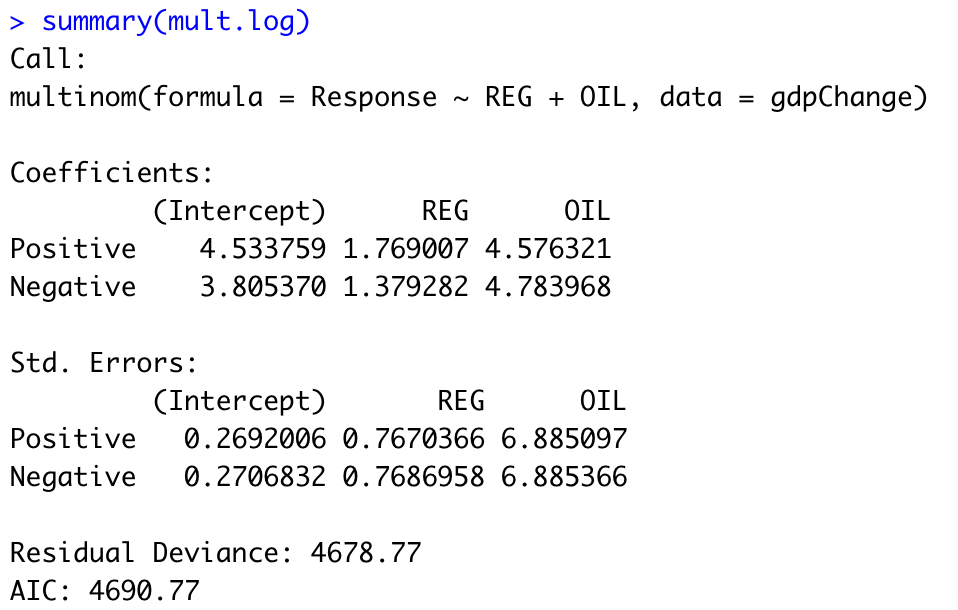
\includegraphics[width=\linewidth]{mult.log.reg}
\\\\

\noindent We can see here the estimated coefficients of the regression, namely \texttt{$REG_p$} = 1.769007, \texttt{$OIL_p$} = 4.576321, \texttt{$REG_n$} = 1.379282  and \texttt{$OIL_p$} = 4.783968.
\\\\
\noindent We can also see the estimated cut off points of $\beta_p$ = 4.533759 and $\beta_n$ = 3.805370.



\pagebreak

\subsection{Interpretation of coefficients}

\noindent g. Interpretation of coefficients: multinomial regression models take the following form: 

\begin{equation}
ln(\frac{p_{i2}}{p_{i1}}) = \beta_{02} + \beta_{12}X_i 
\end{equation}
\begin{equation}
ln(\frac{p_{i3}}{p_{i1}}) = \beta_{03} + \beta_{13}X_i 
\end{equation}

\noindent In these examples, our reference category is \texttt{$p_i$}. This means that our coefficient in the first equation, $\beta_{12}$, is the change in the log odds of going from category 1 to category 2 for a one unit increase in $x_i$, holding all else constant. 
\\\\
\noindent $\beta_{02}$ refers to the intercept of the equation
\\\\
\noindent
Similarly, our coefficient $\beta_{13}$ is the change in the log odds of going from category 1 to category 3 for a one unit increase in $x_i$, holding all else constant.
\\\\
\noindent $\beta_{03}$ refers to the intercept of the second equation.
\\\\
\noindent
We can apply these equations to the coefficients from our multinomial model.
\\\\
\begin{equation}
ln(\frac{p_{iPositive}}{p_{iNoChange}}) = \beta_{0NCtoP} + \beta_{R1}X_{R} + \beta_{O1}X_{O} 
\end{equation}

\noindent 
Using our coefficients from the previous table, we can form the following 

\begin{equation}
ln(\frac{p_{iPositive}}{p_{iNoChange}}) = 4.533759 + 1.769007X_{R} + 4.576321X_{O} 
\end{equation}


\noindent We can also apply our unordered regression model equation to the second coefficients


\begin{equation}
ln(\frac{p_{iNegative}}{p_{iNoChange}}) = \beta_{0NCtoN} + \beta_{R2}X_{R} + \beta_{O2}X_{O}
\end{equation}

\noindent When we input the coefficients from the table, we can get the following equation:

\begin{equation}
ln(\frac{p_{iNegative}}{p_{iNoChange}}) = 3.805370 + 1.379282X_{R} + 4.783968X_{O}
\end{equation}

\pagebreak
\subsubsection {Interpretation of the intercepts}

\noindent We can interpret the intercepts of the regressions as follows:
\\\\
\noindent The log odds that a countries GDP growth will go from 'No change' to 'Positive', when the covariate for \texttt{REG} ($X_{R1}$) is equal to zero  and the covariate for \texttt{OIL} ($X_{O1}$) is equal to zero is 4.533759.
\\\\
\noindent In real terms, 4.533759 is the log odds of that a non-democracy for whom oil is not a majority of their exports will experience a change from "No change" to "Positive" GDP growth. 
\\

\noindent The log odds that a countries GDP growth will go from 'No change' to 'Negative', when the covariate for \texttt{REG} ($X_{R1}$) is equal to zero  and the covariate for \texttt{OIL} ($X_{O1}$) is equal to zero is 3.805370.
\\

\noindent In real terms, 3.805370 is the log odds of that a non-democracy for whom oil is not a majority of their exports will experience a change from "No change" to "Negative" GDP growth.
\\\\


\subsubsection{Interpretation of \texttt{REG} coefficients}


\noindent We can interpret the first \texttt{REG} coefficient $\beta_{R1}$ as follows: a one unit in $X_{R}$ is associated with a 1.769007 increase the log odds that GDP growth will change from "No change" to "Positive" that year, holding all other factors, such as oil exports, constant.
\\

\noindent In real terms, this means that we would expect a 1.769007 increase in the log odds that GDP growth would change from "No change" to "Positive", when looking at democracies versus non-democracies, holding all other factors, such as oil exports constant.
\\

\noindent We can interpret the second \texttt{REG} coefficient $\beta_{R2}$ as follows:  for a a one unit increase in $X_R$, we would expect a 1.379282 increase in the log odds that GDP growth for countries will change from "No change" to "Negative", holding all other factors, such as oil exports, constant.
\\

\noindent In real terms, this means that we would expect a 1.379282 increase in the log odds that GDP growth will change from "No change" to "Negative", when looking at democracies versus non-democracies, holding all other factors, such as oil exports, constant.
\\\\

\subsubsection{Interpretation of \texttt{OIL} coefficients}

\noindent We can interpret the first \texttt{OIL} coefficient $\beta_{O1}$ as follows: a one unit increase in $X_O$ is associated with a 
4.5476321 increase in the log odds that GDP growth for countries will change from "No change" to "Positive", holding all other factors, such as regime type, constant.
\\

\noindent In real terms, this means that we would expect a 4.576321 increase in the log odds that GDP growth will change from "No change" to "Positive", when looking a major oil producers versus non-major oil producers, holding all other factors, such as regime type, constant.
\\

\noindent We can interpret the second \texttt{OIL} coefficient $\beta_{O2}$ as follows: a one unit increase in $X_O$ is associated with a 4.783968 increase in the log likelihood that GDP growth will go from "No change" to "Negative", holding all other factors, such as regime type, constant.
\\

\noindent In real terms, this means that we would expect a 4.783968 increase in the log likelihood that GDP growth will go from "No change" to "Negative", when looking at a major oil producers versus non-major oil producers, holding all other factors, such as regime type, constant. 
\\\\

\subsection{Statistical tests of the coefficients}

\noindent We can calculate z scores by dividing the coefficients by their standard errors. We can then use these z scores to determine the p-values of each of the coefficients. We can use the following code to do so:

\begin{lstlisting}
z <- summary(mult.log)$coefficients/summary(mult.log)$standard.errors
(p <- (1-pnorm(abs(z), 0, 1))*2)
\end{lstlisting}

\noindent We get the following z scores

\begin{center}
	\begin{tabular}{||c c c c||} 
		\hline
		& Intercept & REG  & OIL \\ [0.5ex] 
		\hline\hline
		Positive &16.84156 & 2.306287& 0.6646706 \\ 
		\hline
		Negative &14.05839 & 1.794314 & 0.6948023\\ [1ex] 
		\hline
	\end{tabular}
\end{center}

\noindent We get the following p-values

\begin{center}
	\begin{tabular}{||c c c c||} 
		\hline
		& Intercept & REG  & OIL \\ [0.5ex] 
		\hline\hline
		Positive &0 & 0.02109459 & 0.5062612 \\ 
		\hline
		Negative &0 & 0.07276308 & 0.4871792\\ [1ex] 
		\hline
	\end{tabular}
\end{center}

\noindent From these tables, at an 0.05 alpha level of significance ($\alpha$ = 0.05), we can see that only one of the coefficients, $\beta_{RP}$, has a p-value below 0.05 and is statistically significantly different from zero. In the cases of the other coefficients, there is not enough evidence to reject the null hypothesis that the coefficients are not equal to zero.


\pagebreak
\section{Question 1}
\noindent 
2. Construct and interpret an ordered multinomial logit with \texttt{GDPWdiff} as the outcome variable, with estimated cutoff points and coefficients.

\subsection{Data Wrangling}

\noindent Much of the necessary wrangling for the data, such as converting from string to factor, has already been completed. However, we still need to do a bit.
\\\\
\noindent (a) We start by converting from unordered categorical data into ordinal data. We use the code similar to that from the previous section, using the \texttt{factor()} function with an added \texttt{ordered = TRUE} argument, and with 'Negative' as the lowest category..
\\\\
\begin{lstlisting}
gdpChange$Response <-factor(gdpChange$Response,
	levels = c("Negative",
						"No change",
						"Positive"),
	labels = c("Negative",
						"No change",
						"Positive"),
	ordered = TRUE)
\end{lstlisting}

\subsection{Running the Model}

\noindent (b) We can run the model with the following code

\begin{lstlisting}
ord.log <- polr(Response ~ REG + OIL,
						data = gdpChange,
						Hess = TRUE)

summary(ord.log)
\end{lstlisting}

\noindent This gives us the following output:

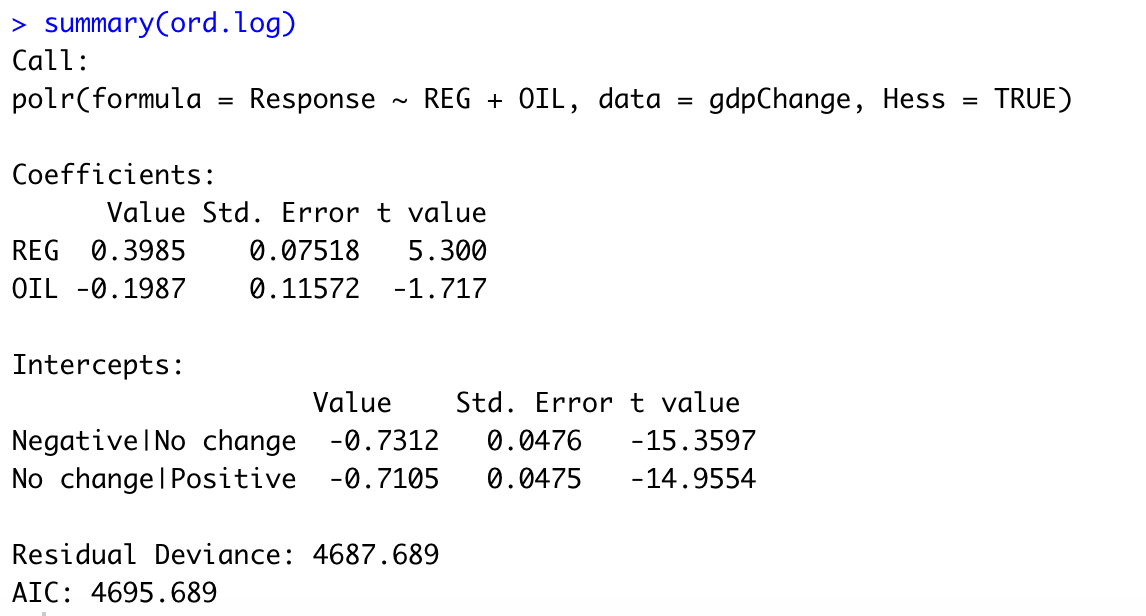
\includegraphics[width=\linewidth]{ordinal.mult.reg}
\\\\

\noindent We can see in this regression table the estimated coefficients for the regression, namely \texttt{REG} = 0.3985 and \texttt{OIL} = -0.1987.
\\\\
\noindent We can also see the cutoff points for the regression, namely \texttt{Negative|No change} = -0.7312 and \texttt{No change|Positive} = -0.7105.

\pagebreak
\subsection{Statistical tests of the coefficients}

\noindent Using the following code we can find p-values for our coefficients:
\\

\begin{lstlisting}
ctable <- coef(summary(ord.log))
p <- pnorm(abs(ctable[, "t value"]), lower.tail = FALSE)*2
(ctable <- cbind(ctable, "p value" = p))
\end{lstlisting}

\noindent Which gives us the following output:
\\

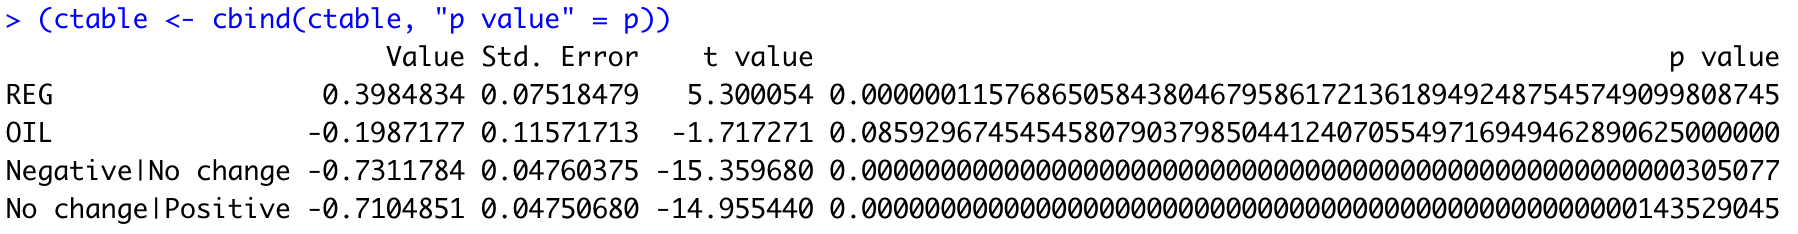
\includegraphics[width=\linewidth]{ord.log.reg2}
\\

\noindent As we can see, at an alpha significance level of 0.05 ($\alpha$ = 0.05), the intercepts for "Negative" to "No change" and "No change" to "Positive", as well as the coefficient for \texttt{REG}, we can reject the null hypothesis that these intercepts and the coefficient are equal to zero (since their p values are below 0.05) and accept the alternative hypothesis that there is a relationship between the \texttt{REG} predictor and the ordinal outcome variable "Response"
\\\\\

\noindent In the case of the coefficient for \texttt{OIL}, at alpha significance level of 0.05 ($\alpha$ = 0.05), we cannot reject the null hypothesis that there the coefficient is equal to zero. We therefore cannot conclude that the \texttt{OIL} variable has an effect on the outcome variable "Response" or leads to a change in the direction of GDP growth.
\\\\

		
\subsection{Interpretation of the coefficients}

\noindent 
When examine the data structure type of the ordinal response variable in R, we get the following output:

\begin{lstlisting}
str(gdpChange$Response)
\end{lstlisting}
\texttt{Ord.factor w/ 3 levels "Negative"<"No change"<..: 3 1 3 3 3 3 1 3 1 3 ...}
\\


\noindent This indicates to us that R has ordered the data in such a way that "Negative" corresponds with 1, "No change" corresponds with 2 and "Positive" corresponds with 3.
\\

\noindent Using the coefficients and cut off points from the ordinal logistic regression table, we can get the estimated model as follows:
\\

\noindent We can calculate the odds ratio for the coefficients, which will allow us to interpret the coefficients, as follow:

\begin{lstlisting}
(ci <- confint(ord.log))
exp(cbind(OR = coef(ord.log), ci))
\end{lstlisting}

\noindent This gives us the following output:
\\\\
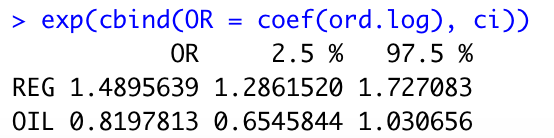
\includegraphics{ord.log.OR}
\\\\
\noindent We can interpret these odds ratios in the following way: for those countries that democracies, the odds experiencing non-negative growth ("No change" or "Positive") is 1.49 times that of countries that are not democracies, holding all other variables constant
\\\\
For those countries that are major oil exporters, the odds of that they will experience non-negative GDP growth ("No change" or Positive) is 19\% lower than non-major oil exporters, holding all other factors constant.



\pagebreak

\section{Question 2}

(a) Run a Poisson regression because the outcome is a count variable. Is there evidence that PAN presidential candidates visit swing districts more? Provide a test statistic and p-value.
\\

\subsection{Theory}

The Poisson regression model is a generalised linear model takes the form

\begin{equation}
ln(\lambda_i) = \beta_0 + \beta_1X_{1i} + \beta_2X_{2i} + ... + \beta_kX_{ki}
\end{equation}

Where

\begin{equation}
\lambda_i = e^{\beta_0 + \beta_1X_{1i} + \beta_2X_{2i} + ... + \beta_kX_{ki}}
\end{equation}

such that ln($\lambda_i$) refers to the natural log of the Poisson parameter $\lambda_i$
\\\\

\subsection{Model 1}

\noindent (a) Our first step is to load in the municipal data, which we do as shown below:
\\
\begin{lstlisting}
muniData <- read.csv("MexicoMuniData.csv")
\end{lstlisting}

\noindent (b) We then test a model whereby \texttt{PAN.visits.06} is the outcome variable and \texttt{competitive.district} is our predictor variable.
\\
\begin{lstlisting}
# Running Poisson model 1
poisson.reg <- glm(PAN.visits.06 ~ competitive.district,
data = muniData,
family = poisson)

summary(poisson.reg)
\end{lstlisting}

\noindent In calling the summary() function, we get the following output.
\\
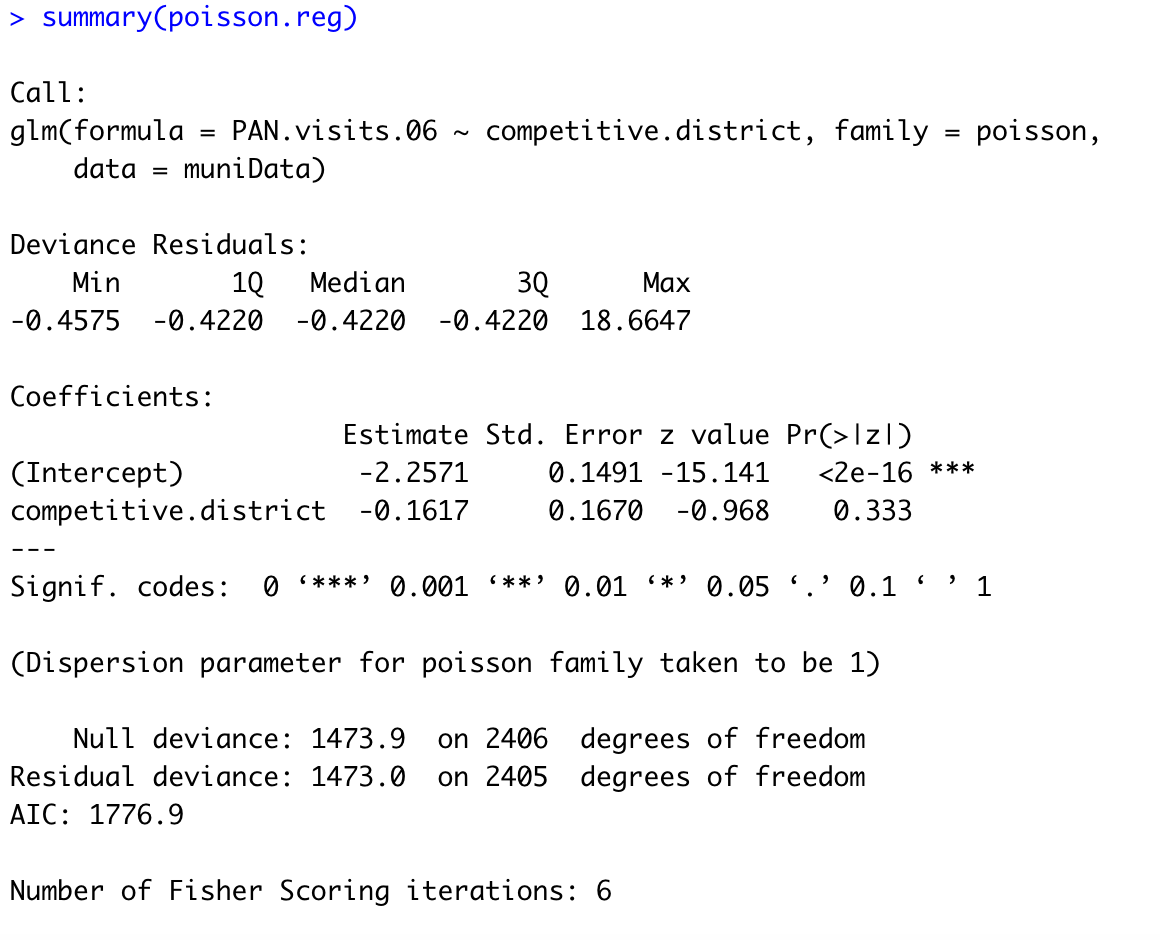
\includegraphics[width=\linewidth]{poisson.model.1}
\\

\subsubsection{Interpretation}
\noindent 
An initial look at this table appears to indicate that the relationship between the outcome variable \texttt{PAN.visits.06} and the predictor variable \texttt{competitive.district} is not statistically significant from zero. In other words there is not enough evidence to suggest that there is a relationship between the two variables based on this model.
\\\\
\noindent We can further test this by looking at the test statistic and a p-value.
\\\\
\noindent
The test statistic, or z value, for the hypothetical coefficient $\beta_{cd}$ is -0.968.
\\

\noindent
The p-value for the coefficient is 0.333. 
\\

\noindent Assuming our alpha level of significance to be 0.05 ($\alpha = 0.05$), there is not enough evidence to conclude that our coefficient for \texttt{$beta_{cd}$} is statistically significant from zero.
\\

\noindent We can therefore cannot conclude that PAN presidential candidates visit swing districts more.
\\\\

\subsection{Model 2}

\noindent (a) We run another Poisson regression model with \texttt{PAN.visits.06} as our outcome variable and \texttt{competitive.district}, \texttt{marginality.06} and \texttt{PAN.governor.06} as our predictor variables. 

\begin{lstlisting}
poisson.reg1 <- glm(PAN.visits.06 ~ competitive.district+
	marginality.06 +
	PAN.governor.06,
	data = muniData,
	family = poisson)
	
summary(poisson.reg1)
\end{lstlisting}

\noindent The summary call gives us the following output:
\\

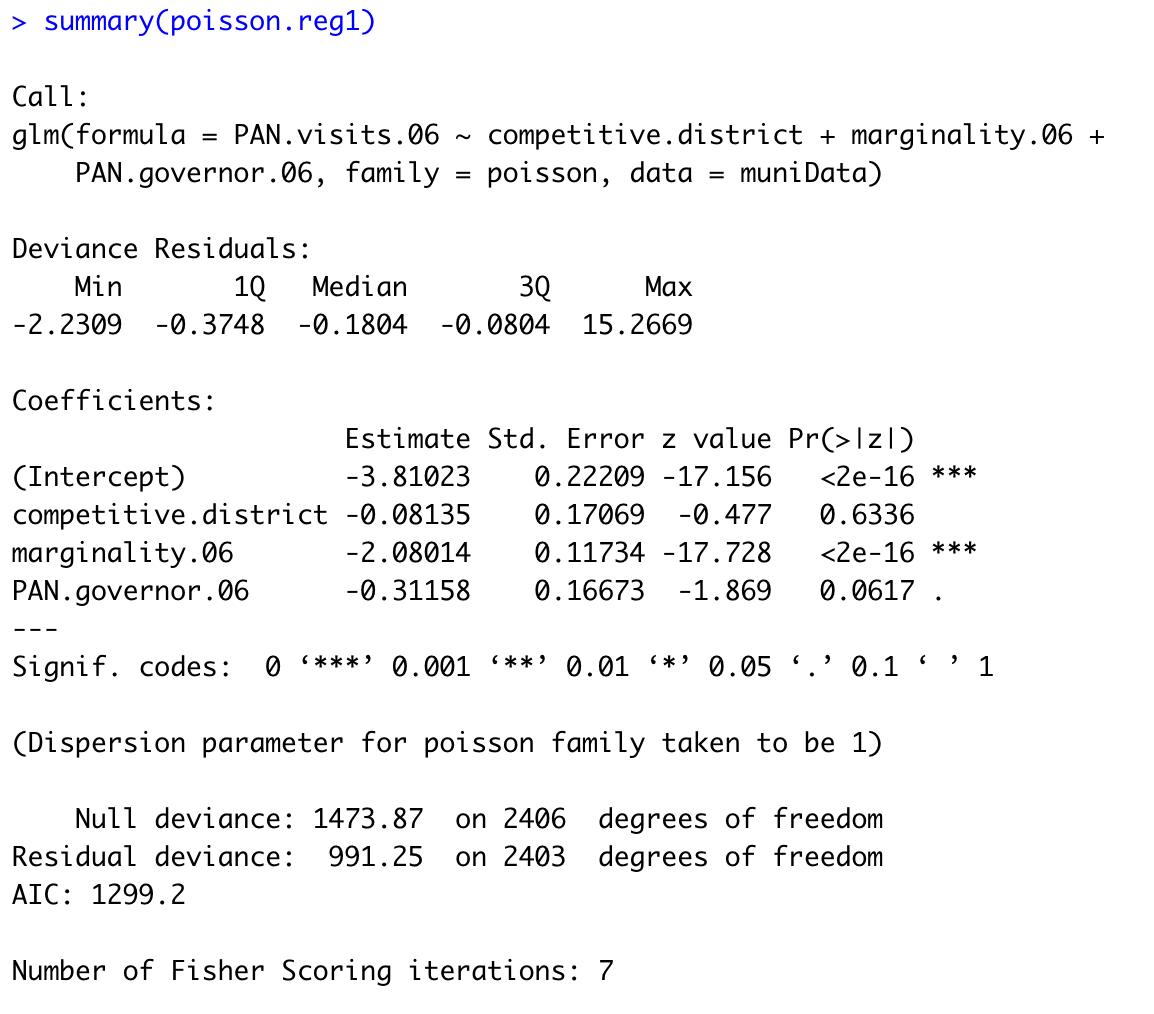
\includegraphics[width=\linewidth]{poisson.model.2}

\noindent We can see from the output of this model that there appears to be statistically significant non-zero relationship between the predictor \texttt{marginality.06} and our outcome variable \texttt{PAN.visits.06}.
\\
\noindent Our test statistic, or z-score, for the coefficient is z = -17.728.
\\

\noindent Our p-value is less than 2e-16. 
\\

\noindent This means that at an alpha level of significance of 0.05 ($\alpha = 0.05$), we can reject the null hypothesis that there is a non-zero relationship between the \texttt{marginality.06} and our outcome variable \texttt{PAN.visits.06}.

\begin{equation}
ln(\lambda) = \beta_0 + \beta_1X_1 + \beta_2X_2 + \beta_3X_3
\end{equation}

\begin{equation}
ln(\lambda) = -3.81023 - 0.08135X_1 - 2.08014X_2- 0.31158X_3
\end{equation}

\noindent As we can see from the table, the coefficient \texttt{competitive.district} has a test statistic of -0.477 and a p-value of 0.6336. Assuming an alpha significance level of 0.05 ($\alpha$ = 0.05), since the \texttt{competitive.district} p-value of 0.6336 is greater than 0.05, there is not enough evidence to conclude that PAN presidential candidates visit swing districts more.




\pagebreak

\noindent (b) Interpret the \texttt{marginality.06} and \texttt{PAN.governor.06} coefficients.
\\\\

\noindent We can interpret our \texttt{PAN.governor.06} coefficient ($\beta_3$) by saying that a one unit increase in the covariate (X) of \texttt{PAN.governor.06} is associated with $e^{\beta_3}$ times more visits by the winning PAN presidential candidates, according to our model. 
\\\\
\noindent We can calculate $e^{\beta_3}$ using the following code:
\begin{lstlisting}
exp(cfs[4])
\end{lstlisting}

\noindent This gives us a result of 0.7322898.
\\\\
This is how many more visits a district with a PAN governor could expect versus a district versus a district without a PAN governor, holding all other factors and assuming that the coefficient is statistically significantly different from 0.
\\\\

\noindent 
If we were to use an alpha significance level of 0.1 ($\alpha = 0.1$), we can use this interpretation, since our p value of 0.0617 is less than 0.1.
\\\\

\noindent However, if we use an alpha significance level of 0.05 ($\alpha = 0.05$), we cannot conclude that there is a not a non-zero relationship between the outcome variable and \texttt{PAN.governor.06}. That is to say, we would not be able to reject the null hypothesis that $\beta_3$ = 0.
\\\\

\noindent We can interpret our \texttt{marginality.06} by saying that for a one unit increase in our predictor variable for \texttt{marginality.06}, we would expect an $e^{\beta_2}$ times more visits according t our model.
\\\\

\noindent We can calculate  $e^{\beta_2}$ with the following code:

\begin{lstlisting}
exp(cfs[2])
\end{lstlisting}

\noindent This gives us a result of 0.9218693. 
\\\\
This is how many more visits a district could expect for a one unit increase in \texttt{marginality.06}, according to our model and holding all other factors constant.
\\\\
It is not fully clear whether a positive marginality score refers to a richer than average or a poorer than average district.
\\\\
Assuming that a positive marginality score refers to richer than average districts, it would mean that we would expect more visits to richer than average areas by the PAN presidential candidate, holding other factors constant.
\\\\
Assuming a positive marginality score refers to poorer than average districts, it means that we would expect more visits to poorer than average districts by the PAN presidential candidate, holding other other factors constant.

\pagebreak
\noindent (c) Interpret the estimated mean number of visits from the winning PAN presidential candidate fora hypothetical district that was competitive (\texttt{competitive.district}=1), had an average poverty level (\texttt{marginality.06}) and a PAN governor (\texttt{PAN.governor.06} = 1).
\\\\
\noindent We can use the following code save the coefficients of the poisson regression. 

\begin{lstlisting}
cfs <- coef(poisson.reg1)
\end{lstlisting}

\noindent Index 1 of \texttt{cfs} corresponds with the intercept of the regression, index 2 corresponds with the coefficient for \texttt{competitive.district}, index 3 corresponds with the coefficient for \texttt{marginality.06} and index 4 corresponds with the coefficient for \texttt{PAN.governor.06}.
\\\\
\noindent With this in mind, we can form a formula to calculate the estimated number of visits with the indices, by multiplying index 2 by 1 (\texttt{competitive.district} = 1), multiplying index 3 by 0 (\texttt{marginality.06}) and multiplying index 4 by 1 (\texttt{PAN.governor.06}).
\\\\
\noindent We can do this by running the following code:

\begin{lstlisting}
exp(cfs[1] + cfs[2]*1 + cfs[3]*0+ cfs[4]*1)
\end{lstlisting}

\noindent With this we get an expected number visits of 0.01494818.
\\



\end{document}
